\chapter[Metodologia]{Metodologia}
\label{ch:metodologia}

Neste capítulo, será apresentada a metodologia utilizada no desenvolvimento dessa 
monografia. Na seção 4.2, será detalhada a classificação de pesquisa, de acordo com os 
critérios de abordagem, natureza, objetivos e procedimentos. A seção 4.3 acordará o fluxo 
das atividades que foram desenvolvidas ao longo do Trabalho de Conclusão de Curso (TCC), considerando duas etapas de dedicação. 
A seção 4.4 abordará a pesquisa bibliográfica.
A seção 4.5 focará na metodologia de desenvolvimento. A seção 4.6 permitirá conhecer como foi conduzida 
a análise de resultados. A seção 4.7 ilustra o cronograma das atividades desenvolvidas ao 
longo desse trabalho. Por fim, têm-se as considerações finais do capítulo.


\section{Classificação da Pesquisa}

De acordo com \citeonline{gerhardt2009}, a metodologia é o estudo da organização dos 
caminhos a serem percorridos para se realizar uma pesquisa, um estudo ou para se 
fazer ciência. No caso de uma pesquisa científica, ela pode ser classificada quanto à 
abordagem; quanto à natureza; quanto aos objetivos, e quanto aos procedimentos.

\subsection{Quanto à Abordagem}

A classificação quanto à abordagem pode ser dividida em: pesquisa qualitativa e quantitativa. 

A pesquisa qualitativa busca explicar o porquê das coisas, e 
comumente analisa dados que não são métricos, tornando difícil 
a quantificação de valores. Ela tende a salientar os
aspectos dinâmicos, holísticos e individuais da experiência humana, para apreender
a totalidade no contexto daqueles que estão vivenciando o fenômeno \cite{gerhardt2009}.

Já a pesquisa quantitativa têm resultados que podem ser quantificados, sendo baseada na 
análise de dados brutos, tendendo a enfatizar o raciocínio dedutivo, as regras da lógica 
e os atributos mensuráveis da experiência humana

\textbf{Tendo o conhecimento desses conceitos, nesse trabalho, a pesquisa é, 
predominantemente, qualitativa, por possuir resultados não métricos que precisam de 
interpretação.} 


\subsection{Quanto à Natureza}

Segundo \citeonline{gerhardt2009}, a pesquisa quanto à natureza pode ser dividida em pesquisa 
básica e pesquisa aplicada. A pesquisa básica gera conhecimentos novos, sem aplicação básica 
prevista, e a pesquisa aplicada gera conhecimentos para aplicação prática, dirigidos à solução de 
problemas específicos. Tendo o objetivo de desenvolver um aplicativo com os conhecimentos 
adquiridos, a pesquisa a ser realizada nesse trabalho é de natureza aplicada.

 
\subsection{Quanto aos Objetivos}

Quanto aos objetivos, \citeonline{gil1991} classifica as pesquisas em exploratória, 
descritivas e explicativas. 

A pesquisa exploratória tem como objetivo o aprimoramento 
de ideias, ou a descoberta de intuições, o que a faz ter um planejamento flexível. 
Essas pesquisas envolvem: (i) levantamento bibliográfico, (ii) entrevistas com pessoas 
que tiveram experiência prática com o problema pesquisado, e (iii) análise de exemplos que 
``estimulam a compreensão''.

Essa monografia é, predominantemente, exploratória, 
por envolver levantamento bibliográfico e questionários com mulheres que têm experiência 
prática com o problema. A própria definição do tema teve em si um caráter intuitivo. 

\subsection{Quanto aos Procedimentos}

\citeonline{gil1991} separa a pesquisa quanto aos 
procedimentos em: experimental; bibliográfica; 
documental; de campo; \emph{Ex-Post-Facto}; 
de levantamento; survey; estudo de caso; 
participante; pesquisa-ação; etnográfica e etnometodológica.

Essa pesquisa, quanto aos procedimentos, pode ser classificada como: pesquisa bibliográfica e 
estudo de caso.
Ela é bibliográfica,tiliza levantamento de referências teóricas já analisadas, 
como livros e artigos científicos. É estudo de caso, por 
ser aplicado à comunidade criada pela própria autora, com 
mulheres com interesse no tema.


\section{Fluxo das Atividades}

O fluxo a seguir foi construído utilizando a notação BPMN, e apresenta 
tanto as atividades já desenvolvidas ao longo da execução 
da primeira etapa do TCC, quanto, quanto as desenvolvidas na segunda etapa do TCC. 
Adicionalmente, os próximos tópicos detalharão de 
forma mais específica cada atividade desse fluxo.

\begin{figure}[ht]
	\caption{Fluxo das Atividades Desenvolvidas no TCC}
	\begin{center}
	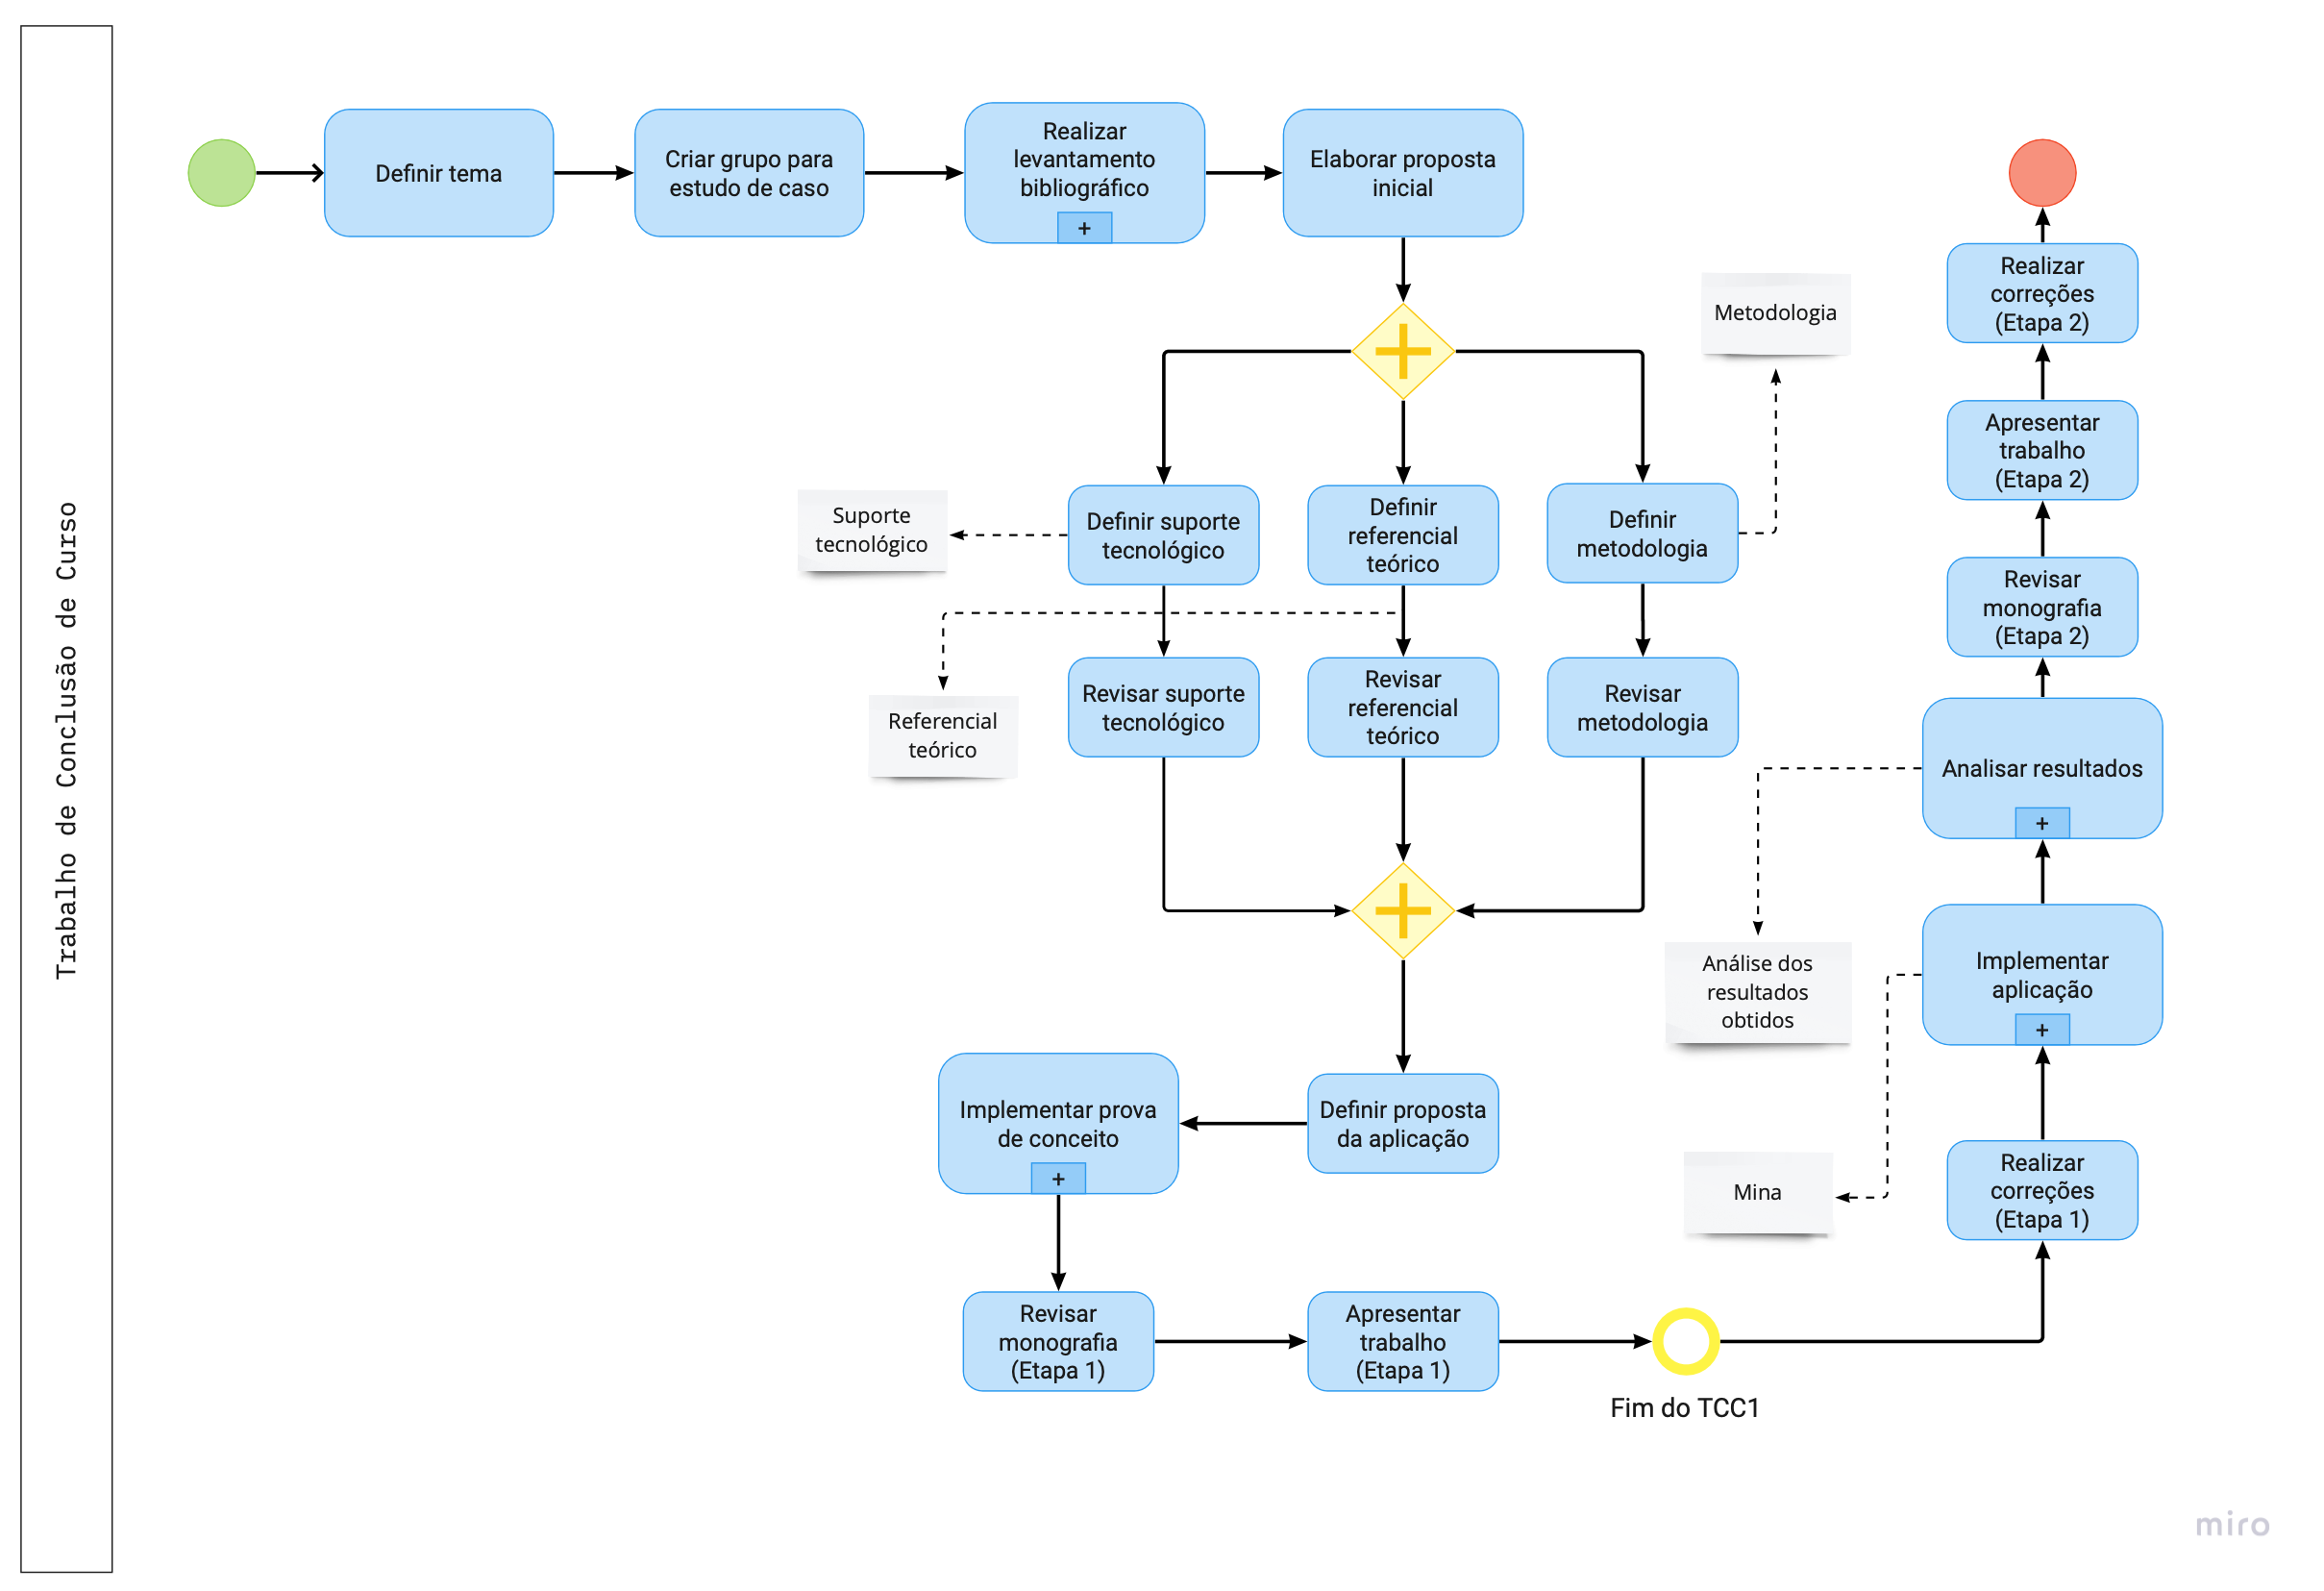
\includegraphics[keepaspectratio=true,scale=0.19]{figuras/fluxodeatividades.png}
	\end{center}
	\legend{Fonte: Autora}
    \label{fig03}
\end{figure}

\textbf{Definir tema}: o tema foi escolhido, junto aos orientadores, utilizando o ciclo 
menstrual como domínio, e discutindo
possíveis aplicações da engenharia de software sobre o tema. 

\textbf{Criar grupo para estudo de caso}: foi criado um grupo com mulheres em idade 
fértil, 
que se interessaram pelo tema e resolveram apoiá-lo. Esse grupo foi utilizado 
para o estudo de caso.

\textbf{Realizar levantamento bibliográfico}: nessa etapa, foi obtido um conhecimento 
inicial do tema, e levantadas publicações pertinentes sobre os tópicos dessa monografia. 

\textbf{Elaborar proposta inicial}: nessa etapa, foi elaborada uma proposta inicial que 
atendesse a necessidade da comunidade, e conciliasse domínio e engenharia de software. 
Optou-se pela criação de um aplicativo com sistema de recomendação de tarefas baseadas 
no perfil e
na fase do ciclo menstrual feminino. No capítulo \ref{ch:mina}, o aplicativo de recomendações de 
tarefa, intitulado Mina, será 
mais bem detalhado.

\textbf{Definir suporte tecnológico}: nessa etapa, foram levantadas as tecnologias necessárias para o desenvolvimento da 
aplicação, gerenciamento do projeto, e pesquisa. Gerou o capítulo \ref{ch:suporte} como artefato.

\textbf{Revisar suporte tecnológico}: o capítulo de suporte tecnológico foi revisado pelos orientadores, e foram implementadas as devidas correções e sugestões.

\textbf{Definir referencial teórico}: nessa etapa, foram levantadas as principais fontes conceituais para embasar o presente trabalho. Gerou o capítulo \ref{ch:referencial} como artefato.

\textbf{Revisar referencial teórico}: o capítulo \ref{ch:referencial} foi revisado pelos orientadores, e foram implementadas as devidas correções e sugestões.

\textbf{Definir metodologia de pesquisa}: nessa etapa, foi definida a metodologia 
para guiar a pesquisa, permitindo classificar essa última quanto
à abordagem, à natureza, aos objetivos, e aos procedimentos. Gerou como artefato o capítulo \ref{ch:metodologia}.

\textbf{Revisar metodologia de pesquisa}: o capítulo de metodologia foi revisado pelos orientadores, e foram implementadas as devidas correções e sugestões.

\textbf{Definir proposta da aplicação}: delimitou-se o escopo da proposta inicial, obtendo um maior detalhamento 
dos objetivos gerais e específicos deste trabalho. Gerou como artefato o capítulo Proposta no 
escopo da primeira etapa. No momento, detallhamento completo do aplicativo encontra-se no capítulo \ref{ch:mina}, Mina.

\textbf{Implementar prova de conceito}: implementou-se parte da proposta, desenvolvendo um protótipo e uma aplicação inicial, com o objetivo 
de avaliar a viabilidade do projeto e das tecnologias escolhidas.

\textbf{Revisar monografia (Etapa 1)}: toda a monografia foi revisada, e as devidas orientações implementadas.
 
\textbf{Apresentar trabalho (Etapa 1)}: apresentar os resultados conquistados, na primeria etapa 
de realização do trabalho, aos membros da banca.

\textbf{Realizar correções (Etapa 1)}: dada as devidas orientações dos membros da banca, correções 
foram realizadas na primeira parte do trabalho.

\textbf{Implementar aplicação}: atividade desenvolvida na segunda etapa do trabalho, 
gerando o aplicativo Mina como artefato.

\textbf{Analisar resultados}: atividade desenvolvida, também na segunda etapa do trabalho, 
com o objetivo de
analisar os resultados obtidos com a implementação da aplicação, conferindo se ela atende 
aos objetivos gerais e específicos estabelecidos no capítulo \ref{ch:intro} desta monografia.

\textbf{Revisar monografia (Etapa 2)}: toda a monografia foi revisada, e as devidas orientações implementadas.
 
\textbf{Apresentar trabalho (Etapa 2)}: apresentar os resultados totais conquistados, na 
realização do trabalho, aos membros da banca.

\textbf{Realizar correções (Etapa 2)}: dada as devidas orientações dos membros da banca, correções 
serão implementadas no trabalho.

\section{Pesquisa Bibliográfica}

A pesquisa bibliográfica foi realizada a partir da plataforma do Periódico Capes, utilizando a ferramenta de pesquisa avançada.
Os temas foram separados em duas partes: influências do ciclo menstrual e sistema de recomendação.
Para as influências do ciclo menstrual, vale ressaltar que é um tema ainda pouco abordado na literatura, e existem 
várias discrepâncias entre os estudos. Dessa forma, foram foram selecionados aqueles que apoiavam a tese de que 
o ciclo influencia de alguma forma as habilidades cognitivas, motoras e sensoriais. 

A partir do periódico capes, foi utilizada a seguinte \emph{string} de busca:
qualquer um que contém \emph{menstrual cycle influence} e qualquer um que contém 
\emph{influence of the phases of the mental cycle}. 

Depois, foi utilizada a ferramenta de filtragem, excluindo artigos que tivessem o tópico, \emph{sex difference} e \emph{male}
, e adicionando artigos que fossem da coleção Scopus, Science ou Pubmed e periódicos revisados por pares. Dessa busca, surgiram 167 artigos.
Desses, o trabalho mais relevante foi o de \citeonline{poroma2014}. A partir desse estudo, foram selecionados, pela referência bibliográfica, estudos que apoiavam 
a teoria de que o ciclo influenciava em algum aspecto a vida das mulheres, ou explicassem de forma mais teórica o funcionamento do ciclo menstrual.


Para o sistema de recomendação, foi utilizada uma pesquisa mais geral, procurando por \emph{recommendation system survey}. Dessa pesquisa, o principal artigo selecionado foi o 
do \citeonline{bobadilla2013}. Por esse artigo, outros estudos foram selecionados, utilizando a referência bibliográfica. Com o andamento da escrita, surgiu a necessidade de buscar
por temas mais específicos, tais como: \emph{Hybrid Recommender Systems}, \emph{Collaborative Filtering} e \emph{Content-based filtering}. A tese de mestrado \cite{mauricio} foi adicionada a partir 
de uma conversa com os orientadores, que citaram o trabalho sobre sistema de recomendação realizado por um deles.


\section{Metodologia de Desenvolvimento}
\label{vsf}
No escopo da primeira etapa do TCC, foi utilizado o Kanban para o gerenciamento das tarefas que foram 
desenvolvidas no decorrer da escrita da monografia, da construção da proposta e do desenvolvimento 
da prova de conceito.

O Kanban é um sistema visual que consiste em um quadro com três colunas: a fazer, em execução e feito (vide Figura \ref{fig04}). 
Dentro das colunas, existem cartões com as tarefas ou ações que precisam ser executadas. As tarefas que devem 
ser desenvolvidas ficam, inicialmente, na coluna do a fazer. Ao começar o desenvolvimento, elas são alocadas para a coluna 
em execução. Quando finalizadas, as tarefas são movidas para a coluna feito.

\begin{figure}[ht]
	\caption{Kanban das Atividades Desenvolvidas na Primeira Etapa do TCC}
	\begin{center}
	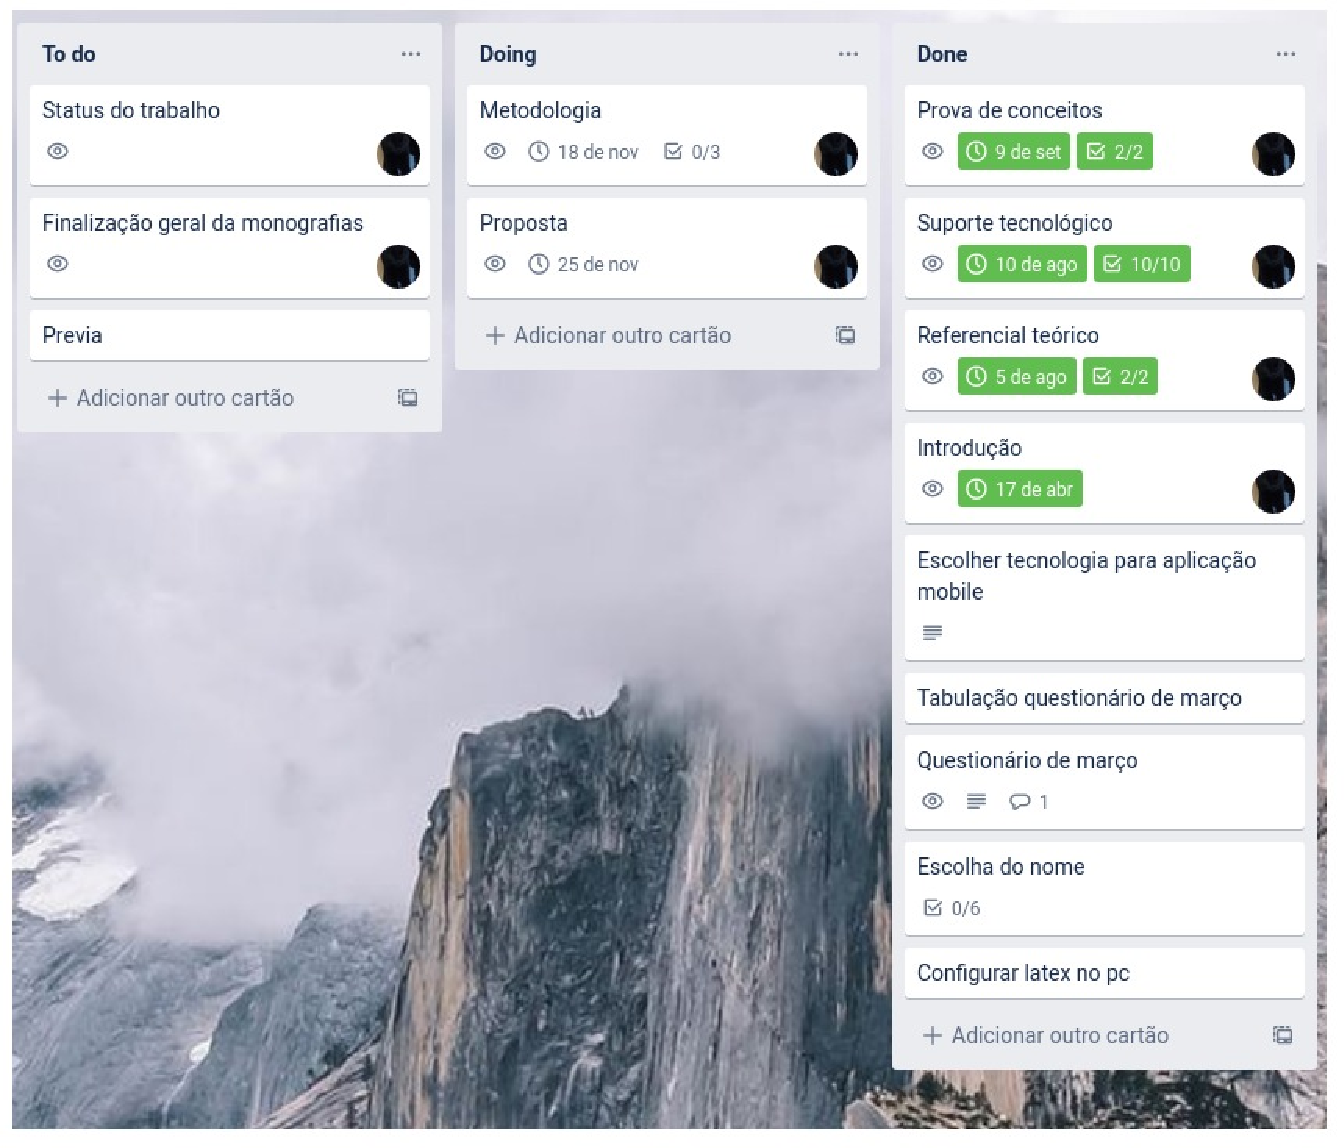
\includegraphics[keepaspectratio=true,scale=0.6]{figuras/kanban.pdf}
	\end{center}
	\legend{Fonte: Autora}
    \label{fig04}
\end{figure}

Na segunda etapa do TCC, foi utilizado um processo baseado em metodologias ágeis, mais especificamente, no Scrum \cite{scrum2017}. O fluxo de desenvolvimento 
pela metodologia Scrum é demonstrado na Figura \ref{fig05}.

\begin{figure}[ht]
	\caption{Metodologia para a Segunda Etapa do TCC}
	\begin{center}
	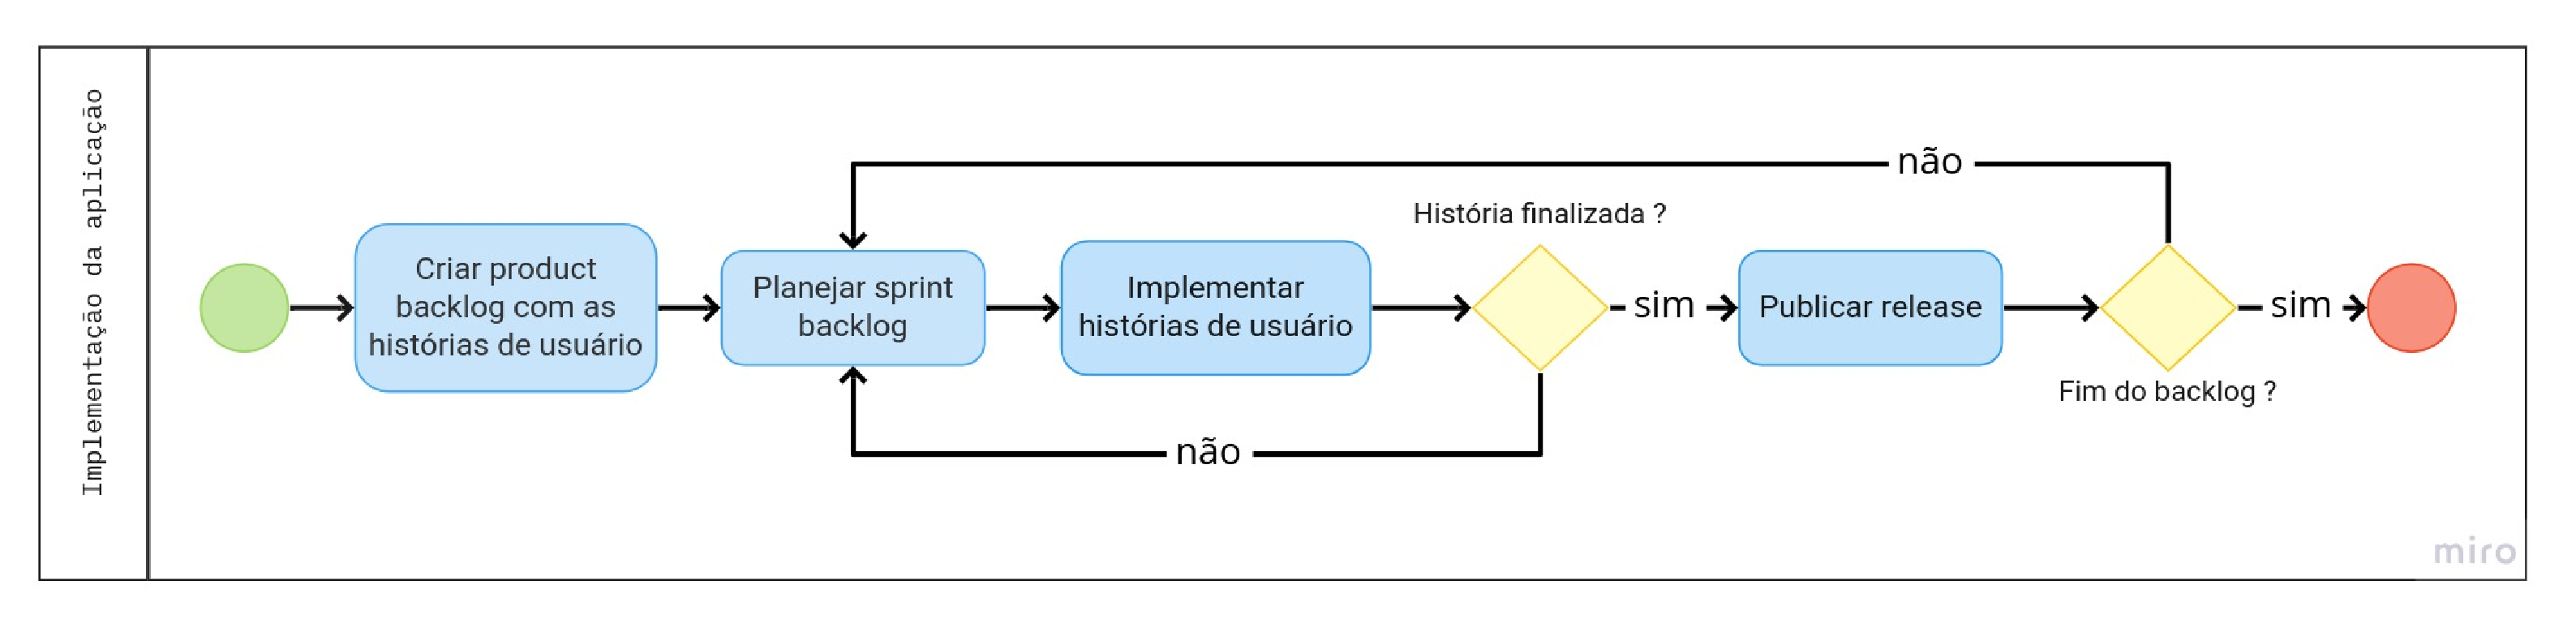
\includegraphics[keepaspectratio=true,scale=0.29]{figuras/scrummet.pdf}
	\end{center}
	\legend{Fonte: Autora}
    \label{fig05}
\end{figure}

\textbf{Criar \emph{product backlog} com as histórias de usuário}: criação do \emph{backlog} separando as histórias de usuário por tema e épico. As histórias de usuário seguiram 
o formato proposto pela metodologia (Eu como ... desejo ... para que eu possa ...). Há ainda critérios de aceitação bem definidos. 

\textbf{Planejar \emph{sprint backlog}}: as histórias de usuário do \emph{product backlog} foram mapeadas para serem executadas durante \emph{sprints} de 15 dias.

\textbf{Implementar história de usuário}: as histórias de usuário foram implementadas e só foram finalizadas quando os critérios de aceitação eram cumpridos.

\textbf{Publicar \emph{release}}: ao final de cada \emph{sprint}, se as histórias de usuário foram executadas, uma nova versão da aplicação é lançada. 

\section{Análise de Resultados}

Segundo \citeonline{gil1991}, o estudo de caso é mais utilizado em estudos exploratórios e descritivos, 
e pode ser importante para fornecer respostas relativas a causas de determinados fenômenos. É definido por sete etapas:
\begin{itemize}
	\item formulação do problema;
	\item definição da unidade-caso;
	\item determinação do número de casos;
	\item elaboração do protocolo;
	\item coleta de dados;
	\item avaliação e análise dos dados; e
	\item preparação do relatório.
\end{itemize}

A formulação do problema foi executada na parte de definição do tema.

A unidade caso é do tipo estudo de caso coletivo. Esse tipo de estudo tem o propósito de estudar características
de uma população, no caso deste trabalho, mulheres em idade fértil.

Para a determinação de números de casos, foram utilizados os múltiplos casos de mulheres em idade fértil que compuseram o grupo de pesquisa criado pela autora. De acordo com o \citeonline{gil1991}, 
o número ideal de casos consiste de quatro a dez casos. O grupo é formado por 22 mulheres inseridas em diferentes contextos.

O protocolo elaborado envolve: visão global do projeto, procedimentos de campo, determinação das questões e guia para a elaboração do relatório.
A visão global do projeto descreve o propósito e o cenário em que foi desenvolvido o estudo. Nesse caso, o propósito é a criação de um aplicativo com sistema de recomendação de tarefas baseadas 
em perfil e fase do ciclo menstrual das mulheres. O cenário em que será desenvolvido o estudo é um grupo criado com mulheres que se interessaram pela proposta do trabalho.

O procedimento de campo envolveu acesso às organizações formadas por mulheres, sendo uma delas o pyladies-df. Através dessas organizações, foi possível mobilizar as mulheres 
para a entrada no grupo do estudo de caso.

A determinação das questões foi feita através de conversas com as 
integrantes do grupo bem como com base nos estudos documentados no 
referencial teórico, capítulo \ref{ch:referencial}. Isso possibilitou a aplicação de 
três questionários para coleta de dados, descritos nos Capítulo 5 e 6.

Por fim, a preparação do relatório deu-se após a aplicação de cada questionário, acordado na etapa anterior.

\section{Cronograma}

O cronograma da Tabela \ref{tab04} explicita as atividades executadas, 
com seus respectivos prazos, na primeira etapa do TCC. A Tabela \ref{tab05} explicita as datas 
de execução inerentes à segunda etapa do TCC. Para fins de uma visualização mais adequada, 
foi considerado com a letra \textbf{P}, a data prevista, e a letra \textbf{E},
para a data Executada.

\begin{table}[ht]
	\centering
	\caption{Atividades da Primeira Etapa do Trabalho}
	\label{tab04}
	
	\begin{tabular}{ccccccc}
		\toprule
		\textbf{Atividades} & \textbf{Março} & 
		\textbf{Julho}  & \textbf{Setembro}& \textbf{Outubro} & \textbf{Novembro} & \textbf{Dezembro}\\
		\midrule
		Definir tema & P-E & & &  &\\
		\midrule
		\begin{minipage} [t] {0.2\textwidth} \centering Realizar Levantamento Bibliográfico \end{minipage} & P-E & E & P & E & & \\
		\midrule
		\begin{minipage} [t] {0.2\textwidth} \centering Elaborar Proposta Inicial\end{minipage} &  & E & P &  &  &\\
		\midrule
		\begin{minipage} [t] {0.2\textwidth} \centering Definir Suporte Tecnológico \end{minipage} & E & P & &  & &\\
		\midrule
		\begin{minipage} [t] {0.2\textwidth} \centering Definir Metodologia de Pesquisa\end{minipage} &  &  & P & E & &\\
		\midrule
		\begin{minipage} [t] {0.2\textwidth} \centering Definir Proposta da Aplicação \end{minipage} &  & & &  & P - E &\\
		\midrule
		\begin{minipage} [t] {0.2\textwidth} \centering Implementar prova de Conceito \end{minipage} &  & E & & E & P-E &\\
		\midrule
		\begin{minipage} [t] {0.2\textwidth} \centering Rever para Revisar Monografia (Etapa 1) \end{minipage} &  & & P-E & P-E & P-E &\\
		\midrule
		\begin{minipage} [t] {0.2\textwidth} \centering Apresentar Trabalho (Etapa 1) \end{minipage} &  &  & &  & & P-E\\
		\bottomrule
	\end{tabular}
\end{table}


O cronograma da primeira etapa sofreu muitas alterações devido à pandemia da Covid-19. O semestre de 2020/1 estava previsto para iniciar no mês de março e finalizar em julho, mas houve uma pausa no 
mês de março, e o retorno ocorreu no mês de agosto. Algumas atividades continuaram sendo desenvolvidas durante essa pausa.



\begin{table}[ht]
	\centering
	\caption{Atividades da Segunda Etapa do Trabalho}
	\label{tab05}
	
	\begin{tabular}{ccccc}
		\toprule
		\textbf{Atividades} & \textbf{Janeiro} & 
		\textbf{Fevereiro}  & \textbf{Março}& \textbf{Abril}\\
		\midrule
		\begin{minipage} [t] {0.2\textwidth} \centering Realizar Correções da Banca \end{minipage} & P/E &  &  &  \\
		\midrule
		\begin{minipage} [t] {0.2\textwidth} \centering Implementar Aplicação \end{minipage} & P & P - E & P - E & P - E  \\
		\midrule
		\begin{minipage} [t] {0.2\textwidth} \centering Análisar Resultados \end{minipage} &  &  &P &P - E  \\
		\midrule
		\begin{minipage} [t] {0.2\textwidth} \centering Refinar Monografia \end{minipage} &  &  &  & P - E \\
		\midrule
		\begin{minipage} [t] {0.2\textwidth} \centering Apresentar Trabalho \end{minipage} &  & & & P - E \\
		\bottomrule
	\end{tabular}
\end{table}

O cronograma da segunda etapa confere as datas de entrega das atividades 
que foram desenvolvidas no semestre de 2021/2. Houve uma diferença de dois semestres entre a execução das etapas, 
o que havia sido acordado à banca, para cumprimento de demais atividades acadêmicas, sendo agravado pela pandemia.

\section{Considerações Finais do Capítulo}

Este capítulo apresentou como o trabalho foi desenvolvido.

As escolhas de classificação dessa pesquisa estão sinalizadas pelos quadros amarelos, Figura \ref{fig06}.

\begin{figure}[ht]
	\caption{Resumo da Classificação da Pesquisa}
	\begin{center}
	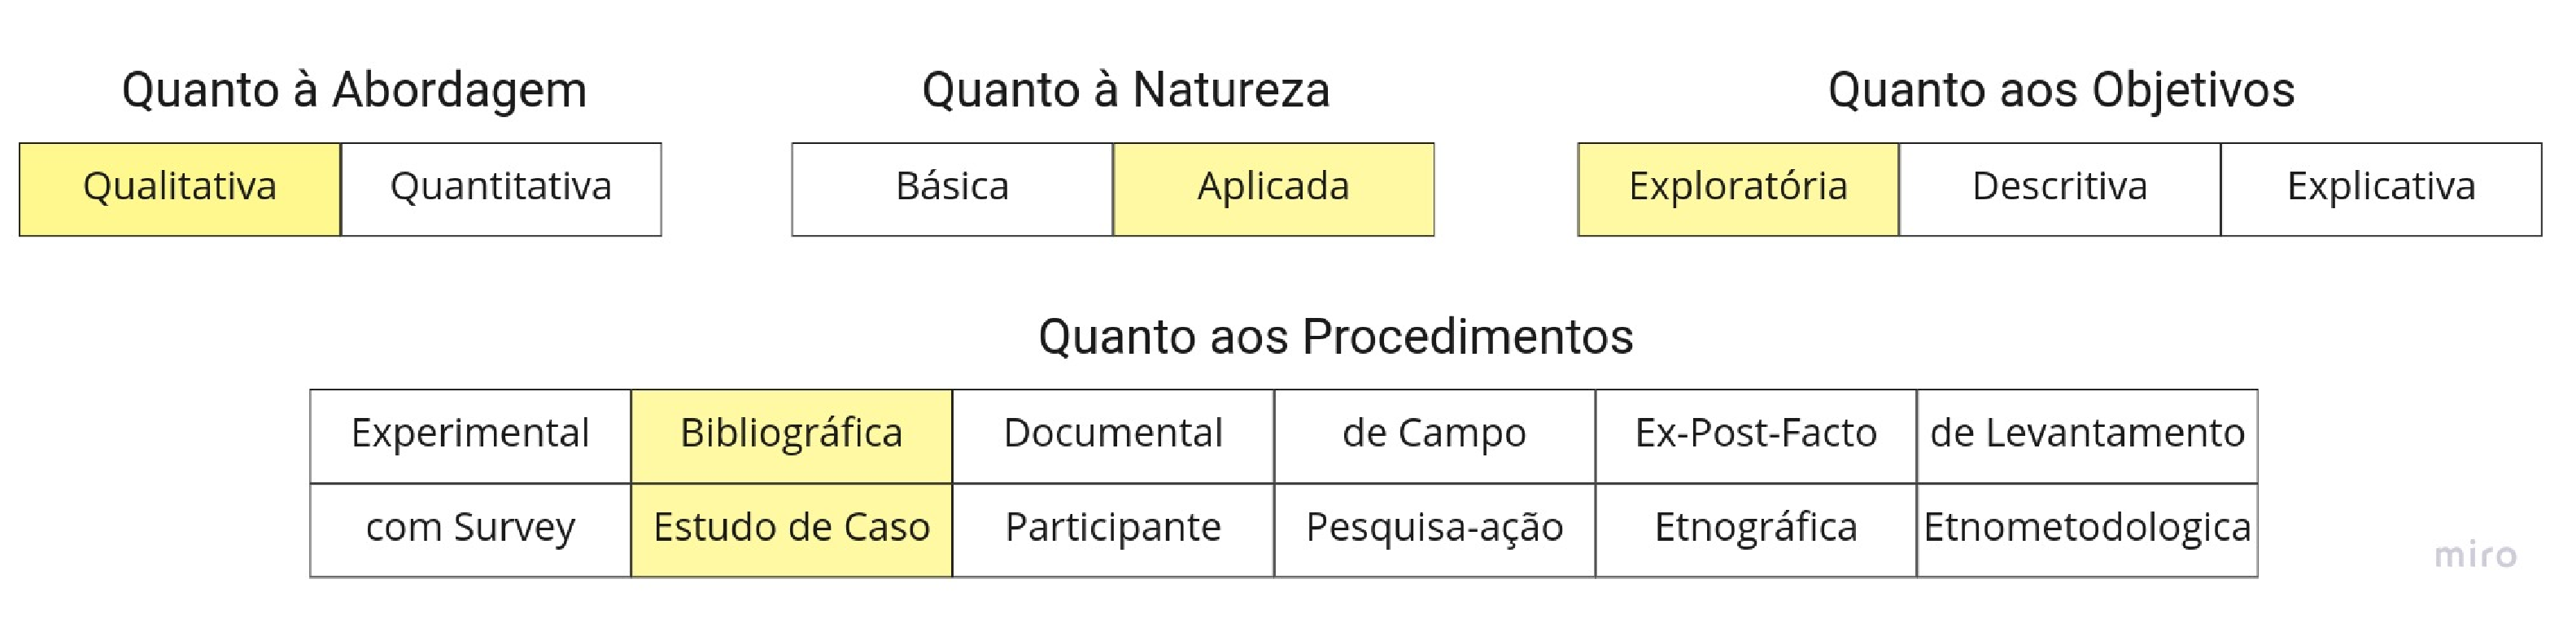
\includegraphics[keepaspectratio=true,scale=0.28]{figuras/resumoAbordagem.pdf}
	\end{center}
	\legend{Fonte: Autora}
    \label{fig06}
\end{figure}

Para o gerenciamento das atividades da primeira etapa do TCC, foi utilizado o Kanban. Como metodologia de desenvolvimento 
para condução da segunda etapa do TCC, foi utilizada uma adaptação do Scrum.

Para a coleta e análise de resultados, foi utilizado um estudo 
de casos aplicado a um grupo de mulheres, sendo esse criado pela 
autora. Cabe ressaltar que a análise de resultados encontra-se mais bem apresentada no Capítulo \ref{ch:capfinal}.



